\documentclass[12pt]{article}
\usepackage{amssymb, amsmath, amsthm, amsfonts}
\usepackage{epic}
\usepackage{eepic}
%\usepackage{hyperref}
\usepackage{listings}
\usepackage{float}
\usepackage{graphicx}
\usepackage{fancyhdr}
\usepackage{color}
\usepackage{enumitem}
\usepackage[letterpaper, margin=1in]{geometry}
\usepackage{mathrsfs}
\usepackage{cleveref}

\newcommand{\C}{\mathbf{C}}
\newcommand{\R}{\mathbf{R}}
\newcommand{\Q}{\mathbf{Q}}
\newcommand{\Z}{\mathbf{Z}}
\newcommand{\N}{\mathbf{N}}
\newcommand{\E}{\mathbf{E}}
\newcommand{\B}{\mathbf{B}}
\newcommand{\F}{\mathbf{F}}
\newcommand{\U}{\mathbf{U}}
\newcommand{\V}{\mathbf{V}}
\newcommand{\J}{\mathbf{J}}
\newcommand{\x}{\mathbf{x}}
\newcommand{\y}{\mathbf{y}}
\newcommand{\z}{\mathbf{z}}
\newcommand{\Ib}{\mathbb{I}}
\newcommand{\Sb}{\mathbf{S}}
\newcommand{\Cs}{\mathscr{C}}
\newcommand{\As}{\mathscr{A}}
\newcommand{\I}{\textnormal{\textbf{I}}}
\newcommand{\Id}{\dot{\textnormal{\textbf{I}}}}
\newcommand{\Top}{\textnormal{\textbf{Top}}}
\newcommand{\hTop}{\textnormal{\textbf{hTop}}}
\newcommand{\Groups}{\textnormal{\textbf{Groups}}}
\newcommand{\Set}{\textnormal{\textbf{Set}}}
\newcommand{\Xib}{\mathbf{\Xi}}
\newcommand{\Sym}{\text{Sym}}
\newcommand{\prid}[1]{\langle #1 \rangle}
\newcommand{\apoly}[1]{a_{#1} + a_{#1}x+ a_{#1}x^2 + \cdots + a_{#1}x^n}
\newcommand{\dist}{\textnormal{dist}}
\newcommand{\ti}[1]{\textit{#1}}
\newcommand{\tb}[1]{\textnormal{\textbf{#1}}}
\newcommand{\es}{\emptyset}
\newcommand{\sst}{\subset}
\newcommand{\ssteq}{\subseteq}
\newcommand{\func}[3]{#1: #2 \to #3}
\newcommand{\inte}[1]{\textnormal{int}(#1)}
\newcommand{\bdr}[1]{\textnormal{bdry}(#1)}
\newcommand{\ifff}{if and only if }
\newcommand{\st}{such that }
\newcommand{\wrt}{with respect to }
\newcommand{\tspace}[1]{\text{T}_#1}
\newcommand{\mathdash}{\hbox{-}}
\newcommand{\diam}[1]{\textnormal{diam}(#1)}
\newcommand{\setst}{\hspace{1mm} | \hspace{1mm} }
\newcommand{\supp}{\textnormal{support}}
\newcommand{\clos}{\textnormal{closure}}
\newcommand{\rel}{\textnormal{rel }}
\newcommand{\Hom}{\textnormal{Hom}}
\newcommand{\obj}{\textnormal{obj}}
\newcommand{\varlisto}[2]{#1_1,#1_2,\ldots,#1_{#2}}
\newcommand{\varlistz}[2]{#1_0,#1_1,\ldots,#1_{#2}}
\newcommand{\finv}[2]{#1^{-1}(#2)}
\newcommand{\disu}{\rotatebox[origin=c]{90}{$\models$}}
\newcommand{\rank}{\textnormal{rank }}
\newcommand{\card}{\textnormal{card }}
\newcommand{\im}{\textnormal{im }}
\newcommand{\cls}{\textnormal{cls }}
\newcommand{\rev}{\textnormal{rev }}
\newcommand{\defeq}{\mathrel{\stackrel{\makebox[0pt]{\mbox{\normalfont\tiny def}}}{=}}}
\newcommand{\Err}{\textnormal{Err}}
\newcommand{\Var}{\textnormal{Var}}
\newcommand{\Ev}{\textnormal{E}}
\newcommand{\pii}[1]{\exp(\beta_{#1}^Tx_i)}
\newcommand{\spii}[1]{\sum_{#1 = 1}^C\exp(\beta_{#1}^Tx_i)}
\newcommand{\spij}[1]{\sum_{#1 = 1}^C\exp(\beta_{#1}^Tx_{i,j})}
\newcommand{\dpp}{\partial}

\renewcommand{\epsilon}{\varepsilon}


\newtheorem*{solution*}{Solution}
\newtheorem{theorem}{Theorem}[section]
\newtheorem{corollary}[theorem]{Corollary}
\newtheorem{proposition}{Proposition}[theorem]
\newtheorem{lemma}[theorem]{Lemma}
\theoremstyle{definition}
\newtheorem*{definition}{Definition}
\newtheorem*{remark}{Remark}
\newtheorem*{remarks}{Remarks}


\renewcommand\qedsymbol{$\blacksquare$}

\author{Luke Meszar}
\date{September 15th, 2017}
\title{CSCI 5622 Homework 1}

\begin{document}
	\thispagestyle{empty}
	
	% --- Header Box --- %
	\newlength{\boxlength}\setlength{\boxlength}{\textwidth}
	\addtolength{\boxlength}{-4mm}
	
	\begin{center}\framebox{\parbox{\boxlength}{\bf
				Machine Learning \hfill Homework 2\\
				CSCI 5622 Fall 2017 \hfill Due Time Sep 29, 2017\\
				Name: Luke Meszar \hfill CU identitykey: lume0018
		}}
	\end{center}
	\section{Logistic Regression (40pts)}																																									
	\begin{solution*}\leavevmode
		\begin{enumerate}[label=\arabic*.,font=\upshape]
			\item \textnormal{What is the role of the learning rate ($\eta$) on the efficiency of convergence during training?}
			\begin{figure}[H]
				\centering
				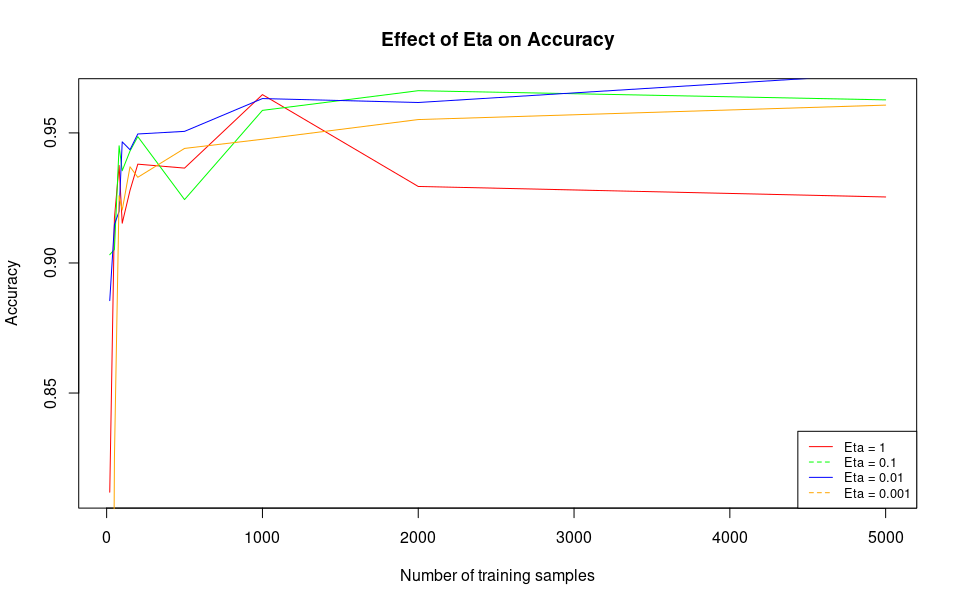
\includegraphics[scale=0.4]{EtaVsAccuracy}
				\caption{Testing how $\eta$ affects accuracy}
				\label{fig:etavsaccuracy}
			\end{figure}
			For small $\eta$, it can take a long time to converge to the minimum. This can be seen by looking at the graph for $\eta = 0.001$. Over 5000 samples, it never reaches the same level of accuracy that $\eta = 0.01$ or ever $\eta = 0.1$ do. However the graph for $\eta = 0.001$ is the smoothest of the four which means that it  follows the gradient of the curve the closest. With a large $\eta$, aka 1, it fails to find the minimum which can be seen by the downward slope at the end of the graph. The accuracy for $\eta = 1$ also jumps a lot at the beginning of the graph showing that it overshooting and then undershooting the minimum. From this graph, it appears that $\eta = 0.01$ is the best choice since it converges the fastest. However, $\eta = 0.1$ would be a better choice if there were fewer samples, say 2200 since the model is more accurate there than for $\eta = 0.01$. 
			\item \textnormal{What is the role of the number of epochs on test accuracy?}
			\begin{figure}[H]
				\centering
				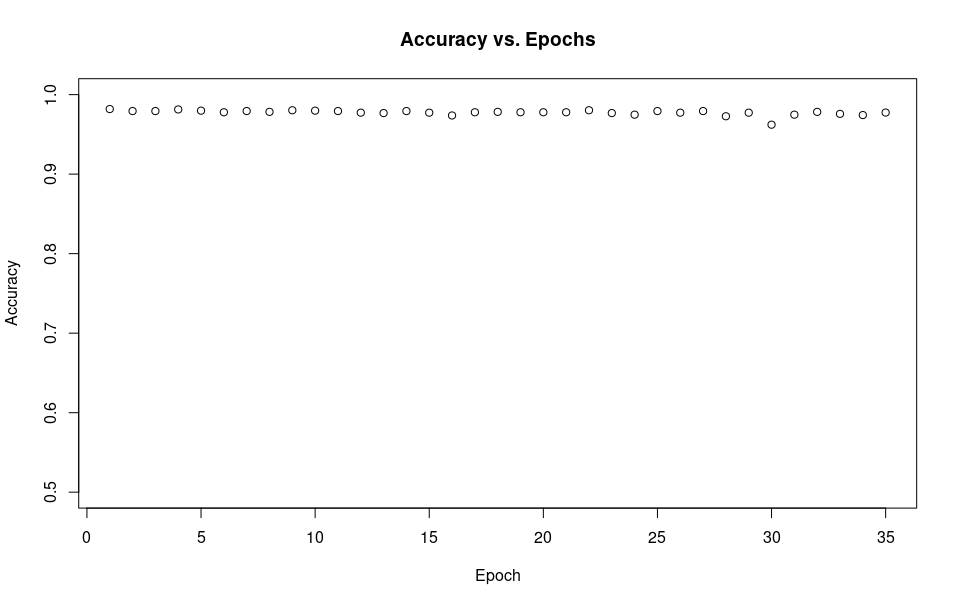
\includegraphics[scale=0.4]{EpochVsAccuracy}
				\caption{Testing how the number of epochs affects accuracy with $\eta = 0.1$}
				\label{fig:epochvsaccuracy}
			\end{figure}
			From \cref{fig:epochvsaccuracy} it is clear that the number of epochs has almost no effect on accuracy. There is some noise in the data, but for the most part, the accuracy is constant with respect to the number of epochs. This makes sense considering the size of an epoch is 9830. From \cref{fig:etavsaccuracy} we see that the accuracy at $\eta = 0.1$ evens out at 5000. Thus, the model is already been trained as well as it can before even finishing one epoch so increasing the number of epochs doesn't affect anything. The reason you may want to use more epochs is it removes some random variations that are possible if the model is only trained once. 
		\end{enumerate}
	\end{solution*}
	\section{Feature Engineering (40 points)}
	\begin{solution*}\leavevmode
		\begin{enumerate}[label=\arabic*.,font=\upshape]
			\item \textnormal{What custom features did you add/try (other than n-grams)? How did those additional features
				affect the model performance? Why do you think those additional features helped/hurt
				the model performance?} 
			
			I added four additional features which were tf-idf, most common suffixes, positive words, and negative words. The tf-idf feature was implemented using scikit-learn's TfidfVectorizer function. This feature was the most successful causing the accuracy to raise to 82.5\%. This feature counts the number of times a word appears in a review and weights it against the frequency of that word occurring in all reviews. Essentially, weights common words low since they do not provide very much information. This is a good measure of which words are important for classification since tf-idf tries to find meaningful words. 
			
			The next feature I tried was looking at the most common suffixes. Given a list of common suffixes, the percentage of words in a review that ended in a common suffix were calculated. This was the least useful feature only increasing the accuracy of the model by 7\%. This is not surprising since it does not seem like a very useful feature. Since the most common suffixes were used, a lot of words will end in them regardless of any sentimental value they may have. Thus, this features measures nothing about the likelihood of a review being positive or negative. 
			
			The final two features I added were similar; calculating the percentage of positive and negative words in a review. Both features increased the accuracy of the model. Due to their similarity, I will only discuss the negative words feature. For each review, the percentage of words that matched one of the negative words in a list was calculated. This is seems like it should be a useful feature since negative reviews are more likely to have negative words. Interestingly, changing the size of the list of negative words affected the accuracy. In a list with 43 word, the accuracy was around 62\% but with a list of only 14 words, the accuracy increases to 66\%. Similar differences were found with the positive words feature. 
			
			\item \textnormal{What are unigrams, bigrams, and n-grams? When you added those features to the FeatureUnion,
				what happened to the model performance? Why do these features help/hurt?}
			
			An n-gram splits a piece of text into groups of n consecutive words. A unigram splits text into sets of one consecutive word, or what would more commonly be called a bag of words. A bigram will split the text into pairs of consective words. When these feature were added, the accuracy on the test data improved from around 50\% at the baseline to 80\%. Adding n-gram features to our model improved performance since reviews in common should have similar word structures. For instance, positive reviews are likely to have words like ``good'', ``great'', ``excellent,'' and ``wonderful.'' Then, the model is trying to predict on a test review, if the review contains words like that, then it is will predict that the review is positive. Adding bigrams and longer n-grams gives more power to this method until it hits diminishing returns. For instance, adding bigrams allows the model to see phrases like ``not good'' which may look like an indicator of positive review if there were only unigrams. However, if n gets too large, then the n-grams will be too specific to the review and will lead to overfitting the data. 
		\end{enumerate}
	\end{solution*}
\section{ Gradient Descent Learning Rule for Multi-class Logistic Regression (20 pts)}
	\begin{solution*}\leavevmode
		\begin{enumerate}[label=\arabic*.,font=\upshape]
			\item \textnormal{Derive the negative log likelihood for multi-class logistic regression.}
			
			Let 
			\[l(\beta) = \prod_{i=1}^{N}\prod_{c=1}^{C} p \left(y_i = c \setst x_i; \beta\right)\]
			be the likelihood function. Then, the negative log likelihood function is
			\begin{align*}
			-\log l(\beta) &= -\left(\sum_{i=1}^{N}\sum_{c=1}^{C} \log p \left(y_i = c \setst x_i; \beta\right)\right) \\
			&= \left[-\sum_{i=1}^{N}\sum_{c=1}^{C} \Ib(y_i = c)\log \frac{\pii{c}}{\spii{c'}}\right]
			\end{align*}
			where $\Ib$ is an indicator function that is 1 when $y_i = c$ and 0 otherwise. Then, using properties of logarithms, we get
			\[\mathscr{L} = -\sum_{i=1}^{N} \left[\left(\sum_{c=1}^{C} \Ib(y_i = c) \beta_c^Tx_i\right) - \log \left(\spii{c'}\right)\right]\]
			
			The term $\left(\sum_{c=1}^{C} \Ib(y_i = c) \beta_c^Tx_i\right)$ can be simplified to $\beta_{y_i}^Tx_i $ since only one of the terms will be nonzero when $y_i = c$. Thus, the simplified log-likelihood function is
			\[ -\sum_{i=1}^{N} \left[\left(\beta_{y_i}^Tx_i\right) - \log \left(\spii{c'}\right)\right]\]
			
			\item \textnormal{The gradient descent learning rule for optimizing weight vectors generalizes to the following form: $\beta^{t+1}_j = \beta^t_j - \eta \nabla \beta^t_j$ where $\eta$ is the learning rate. Find the $\nabla\beta_{c,j}$ (the parameter for
				feature $x_j$ in class $c$) for a multi-class logistic regression model.}
			
			To compute $\nabla\beta_{c,j}$ we compute $\frac{\partial \mathscr{L}}{\partial \beta_{c,j}}$.
			Then
			\begin{align*}
			&\frac{\dpp}{\dpp \beta_{c,j}}\left[ -\sum_{i=1}^{N} \left(\left(\beta_{y_i}^Tx_{i,j}\right) - \log \left(\sum_{c'=1}^C\beta_{c',j}x_{i,j}\right)\right)\right] \\
			&= -\sum_{i=1}^N \frac{\dpp}{\dpp \beta_{c,j}} \beta_{y_i}^Tx_i + \frac{\dpp}{\dpp \beta_{c,j}} \log \left(\spij{c'}\right)\\
			&= -x_{i,j} + \frac{x_{i,j}\exp(\beta_{c,j}x_{i,j})}{\sum_{c'=1}^C\beta_{c',j}x_{i,j}}\\
			&= x_{i,j}\left[-1+p(y = c \setst x)\right].
			\end{align*}
			And thus we have computed  $\nabla\beta_{c,j}$. 
		\end{enumerate}
	\end{solution*}
\end{document}